% ICASSP 2027 submission -- named (single-blind review). Built on venue/paper_kit/Template.tex
% preamble: article + spconf.sty + IEEEbib.bst. Do not regenerate the class.
\documentclass{article}
\usepackage{spconf,amsmath,amssymb,graphicx,url}
\usepackage{booktabs}
\usepackage{microtype}
\usepackage[hidelinks, pdftitle={DD-Koopman: Compact Spectral Transfer for Multi-Step CSI Prediction}, pdfauthor={Jiaxin Liu}]{hyperref}

% --- notation shortcuts -----------------------------------------------------
\newcommand{\Hm}{\mathbf{H}}
\newcommand{\Dd}{\mathbf{D}}
\newcommand{\cc}{\mathbf{c}}

% tight float separation: keeps the added ablation table inside 4 body pages
\setlength{\textfloatsep}{6pt plus 2pt minus 3pt}

\title{DD-Koopman: Compact Spectral Transfer for Multi-Step CSI Prediction}

\name{Jiaxin Liu}
\address{Nanjing University}

\begin{document}
\ninept
\maketitle

\begin{abstract}
Multi-step channel state information (CSI) prediction must balance
forecasting accuracy against inference cost. We propose DD-Koopman, a
compact predictor that cleans the observed history, lifts it into the
delay--Doppler plane, and evolves it there: its poles and per-mode gains
are generated from the observation; the diagonal core is fixed across
horizons and satisfies an exact semigroup law. A calibrated
finite-window readout with zero-gated corrections completes the model. A
closed-form analysis separates input cleaning, spectral propagation and
readout calibration. On the official TDD grid it reaches 0.1402 mean NMSE
against the 21.9M-parameter reference's 0.1246, with 126.5$\times$ fewer
parameters and 4.98$\times$ lower latency. Across three seeds it improves
mean NMSE on unseen propagation, each paired 95\% CI below zero.
DD-Koopman is a compact
alternative to generic CSI backbones with a structured spectral
parameterization.
\end{abstract}

\begin{keywords}
Channel prediction, CSI, operator learning, delay--Doppler, parameter efficiency
\end{keywords}

\section{Introduction}
\label{sec:intro}

The CSI prediction task is to forecast the next four channel states from
sixteen historical observations on a
$4{\times}4{\times}2$ MIMO array over 300 subcarriers; adaptive
modulation, handover and beam management consume its output. The
CSI-4CAST benchmark~\cite{csi4cast_2025} standardises the
splits and the metric and publishes a reference model that reaches a mean
normalised mean square error (NMSE) of 0.1246 on its official 162-setting
TDD-regular grid, at the cost of 21{,}913,750 parameters. Our harness
reproduces the published
number within $0.105\%$ (the benchmark does not seed its RNG), so every
comparison below runs on the same protocol.

Prior work treats the delay domain as an input feature for a generic
backbone: the delay-domain view enters as features or a side branch,
while the multi-step evolution on top remains a generic sequence model.

DD-Koopman instead places the evolution operator itself in the
delay--Doppler plane. A specular
channel is a finite sum of complex exponentials; when each component has constant
Doppler over the observation window, its one-slot evolution is
multiplication by a complex exponential, so the exact predictor is diagonal
in that plane. The classical zero-training DFT-grid extrapolator cannot
express off-grid Doppler, decaying components or the scene-dependent
scattering that sets each mode's radius; DD-Koopman cleans the
observation first and learns all three from it.

Our contributions are:
\begin{enumerate}\itemsep1pt
\item \textbf{Compact observation-conditioned spectral transfer.} We place
the evolution operator in the delay--Doppler plane: a diagonal core
$K_c$ whose poles and per-mode readout gains are generated from the CSI
history, preceded by a residual denoiser and delay-aware input processing
(173{,}190 parameters). Held fixed across horizons, the core satisfies an
exact local semigroup with non-expansive powers; the classical DFT-grid
extrapolator appears as its unit-radius, zero-offset limit, and training
starts from a ridge least-squares spectral warm start on the grid.
\item \textbf{An analysis that separates the three error sources.} For the
diagonal operator we derive a closed-form bound that splits multi-step
prediction error into input-cleaning, propagation and readout-calibration
terms, with the single-mode phase law as a special case; a representation
proposition shows why a grid-pinned retrain can recover the reported
accuracy (\S\ref{ssec:ablations}).
\item \textbf{A validated accuracy--efficiency operating point.} DD-Koopman
reaches 0.1402 mean NMSE against the published reference's 0.1246 while
using 126.5$\times$ fewer parameters and running 4.98$\times$ faster; the width
scan holds competitive accuracy from 58k to 327k parameters, while
shrunk and parameter-matched alternative architectures do not reach this
range. Across three seeds the model
improves mean NMSE on a 432-setting unseen-propagation slice, each paired
CI entirely below zero (\S\ref{ssec:main}, \S\ref{ssec:shift}).
\end{enumerate}

\section{Related Work}
\label{sec:related}

\textbf{Benchmark and published baselines.}
CSI-4CAST~\cite{csi4cast_2025} provides the training grid, the three test
splits, the harness, and the published reference rows we compare against,
including the language-model-based predictor LLM4CP~\cite{llm4cp_2024}. Neural channel
prediction and feedback predate the
benchmark~\cite{oshea2017physical,wen2018csinet,lu2020crnet}. Cross-paper NMSE is not comparable, so we use the benchmark's published reference rows and re-implement the Table~\ref{tab:main} models through its harness.

\textbf{Delay-domain representations and conditioned spectral evolution.}
OTFS~\cite{hadani2017otfs} made the delay--Doppler plane the modulation
domain, exploiting the same sparsity.
Prior work uses the delay domain as an input representation or a
side branch: ChannelKAN~\cite{channelkan_2026} expands dual-domain features
via IDFT, MambaCSP~\cite{mambacsp_2026} embeds a delay-domain
representation next to the frequency view,
PCGAE-Net~\cite{pcgae_2026} crops to the strongest delay taps, and
CSI-BERT2~\cite{csibert2_2024} operates on standard representations of
the same history. We instead make the plane the space where the
operator is diagonal.

\textbf{Dynamics-based and state-space prediction.}
The Koopman programme lifts nonlinear dynamics to linear evolution of
observables~\cite{koopman1931,mezic2005,brunton2017havok}, approximated
from data by extended dynamic mode
decomposition~\cite{williams2015koopman}, deep
embeddings~\cite{lusch2018koopman} and neural
operators~\cite{lu2021deeponet,li2021fno}.
Structured state-space
models~\cite{gu2022s4,smith2023s5}, selective
variants~\cite{mamba_2023} and gated
recurrences~\cite{orvieto2023lru}, with CSI
adaptations~\cite{mambacsp_2026,cpmamba_2025}, learn input-dependent recurrences
in latent coordinates. Our operator is diagonal in an explicit
delay--Doppler basis, and we measure what one frozen model retains under
shift.

\textbf{Efficient forecasting backbones.}
PatchTST~\cite{patchtst_2023}, iTransformer~\cite{itransformer_2024},
TimeMixer~\cite{timemixer_2024}, TSMixer~\cite{tsmixer_2023},
Informer~\cite{zhou2021informer}, N-BEATS~\cite{oreshkin2020nbeats} and
Mamba~\cite{mamba_2023} provide generic forecasting baselines; we
port, retrain and score them under the budgets stated in
Table~\ref{tab:main}, alongside the attention~\cite{vaswani2017attention},
recurrent~\cite{hochreiter1997lstm,cho2014gru} and
linear~\cite{zeng2023dlinear} families
they grew from.

\section{Method}
\label{sec:method}

Per antenna, the history is $\Hm \in \mathbb{C}^{16\times 300}$ (16
slots, 300 subcarriers); the target is the next four slots;
Fig.~\ref{fig:arch} gives the signal path.

\textbf{Lift.} Two parameter-free transforms map the observation into the
working basis:
$a = \mathrm{IDFT}_{\mathrm{sub}}(\Hm)$ converts each slot to its delay
profile (300 taps), and $\Dd = \mathrm{DFT}_{\mathrm{time}}(a)$ converts
along time, giving the delay--Doppler plane. A specular channel concentrates
in a few delay taps and few Doppler modes, so the dynamics live in a
sparse, physically derived coordinate system; the lift has no parameters,
and all 173{,}190 parameters belong to the operator, the residual
denoiser, and the gated correction paths. Concretely: a layer-normalised
log-power context feeds two MLP heads ($16{\to}64{\to}32$ for the 16
pole offsets and radius shifts, $16{\to}64{\to}128$ for the $4{\times}16$
complex gain corrections); a three-filter residual denoiser plus
the two gated paths carry the remainder.

\textbf{Diagonal operator with conditioned eigenvalues.}
For horizon $h \in \{1,\dots,4\}$ (target slot $15{+}h$), the base
prediction extrapolates each mode exponentially:
\begin{equation}
\hat a[h,l] \;=\; \sum_{m} G_h[m](\cc)\; \Dd[m,l]\; \zeta_m(\cc)^{\,h},
\label{eq:operator}
\end{equation}
where $m$ indexes the 16 Doppler bins, $l$ the 300 delay taps, and applying
$\mathrm{DFT}_{\mathrm{sub}}$ to $\hat a$ reconstructs the predicted
frequency-domain CSI. The poles are
$\zeta_m(\cc) = r_m(\cc)\,e^{j2\pi(m+\varepsilon_m(\cc))/16}$ with total
offset $\varepsilon_m(\cc) = \delta_m + \Delta_m(\cc)$: a learned static
offset $\delta_m$ plus an observation-conditioned shift $\Delta_m(\cc)$,
each in $(-\tfrac12,\tfrac12)$, so $\varepsilon_m(\cc)$ places every pole
continuously between the DFT bins. Both the radii $r_m(\cc) \in (0,1)$
and the offsets depend on the observation through a context $\cc$ that
summarises the observed Doppler power averaged over delay taps; the core
$K_c = \mathrm{diag}(\zeta_m(\cc))$ is held fixed across the four
horizons. The gains $G_h[m](\cc)$ are complex, indexed by horizon and
mode, shared across delay taps, and modulated per observation from the
same context; they calibrate the finite-window readout, while the
semigroup property belongs to $K_c$ alone.

\textbf{Proposition 1 (grid limit and stability).} If every component's
Doppler lies on the 16-point grid and stays constant over the window, the
canonical readout $g_m = \tfrac{1}{16}\,e^{j2\pi\cdot 15m/16}$ with
unit-modulus poles reproduces the channel exactly at every horizon
through \eqref{eq:operator}: the grid predictor is the architecture's
unit-radius, zero-offset limit. The reported model initializes its
angular offsets on this grid ($\delta_m$ and $\Delta_m(\cc)$ both start
at zero) and then applies the ridge spectral warm start described below.
For the learned core, $0 <
r_m(\cc) < 1$: the semigroup law $K_c^{\,h+k} = K_c^{\,h}K_c^{\,k}$ holds
exactly and every power is non-expansive, $\|K_c^{\,h}\|_2 \le 1$ ---
stability, not the exact recovery of the unit-radius grid limit.

\textbf{Proposition 2 (fixed-grid expressivity).} Pin the poles to any
nonzero values and disable the gain conditioning: setting
$G_{hm} = (PF_N^{-1})_{hm}\,\zeta_m^{-h}$ makes \eqref{eq:operator}
realise any time map $P \in \mathbb{C}^{H\times N}$ shared across delay
taps, so a grid-pinned model with free per-horizon gains spans every
shared linear multi-step predictor.

\textbf{Theorem 1 (error chain).} Fix the context and compare the
operator's $h$-step action $\widehat A_h = G_h \widehat K^{\,h} \widehat Z$
against a reference decomposition
$A_h^{*} = G_h^{*} K_*^{\,h} Z_*$ of the same coordinates, where
$\widehat Z$ is the lifted, denoised history the operator is fed,
$Z_*$ its ideal counterpart, and
$\|\widehat K\|_2, \|K_*\|_2 \le \rho \le 1$. Then
\begin{equation}
\begin{split}
\|\widehat A_h - A_h^{*}\|_F \;\le\;
\|G_h\|_2 \rho^h e_Z
+ \|G_h\|_2\, h\rho^{h-1} e_K \|Z_*\|_F \\
+ e_G\, \rho^h \|Z_*\|_F,
\end{split}
\label{eq:errchain}
\end{equation}
where $e_Z = \|\widehat Z - Z_*\|_F$, $e_K = \|\widehat K - K_*\|_2$ and
$e_G = \|G_h - G_h^{*}\|_2$: add and subtract $G_h \widehat K^{\,h} Z_*$
and $G_h K_*^{\,h} Z_*$, then expand
$\widehat K^{\,h} - K_*^{\,h} = \sum_{j=0}^{h-1}
\widehat K^{\,h-1-j} (\widehat K - K_*) K_*^{\,j}$, which requires no
commutativity. The three terms are the three design roles: input
cleaning controls $e_Z$, pole placement controls $e_K$, and readout
calibration controls $e_G$. The conditioned heads add a
context-variation term on top of \eqref{eq:errchain} when the context
itself is input-dependent (measured net in \S\ref{ssec:ablations}).

\textbf{Corollary 1 (single-mode phase law).} For one mode where
$\widehat K = \zeta$ and $K_* = \widetilde{\zeta}$ share the radius $r$,
the propagation
difference in \eqref{eq:errchain} is exactly
\begin{equation}
\bigl|\zeta^h - \widetilde{\zeta}^{\,h}\bigr|^2 \;=\; 4\,r^{2h}
\sin^2\!\Big(\frac{\pi h\,(\varepsilon-\widetilde{\varepsilon})}{16}\Big),
\label{eq:sensitivity}
\end{equation}
(substitute $\zeta = r\,e^{j2\pi(m+\varepsilon)/16}$,
$\widetilde{\zeta} = r\,e^{j2\pi(m+\widetilde{\varepsilon})/16}$ and use
$|e^{jx}-e^{jy}| = 2|\sin\frac{x-y}{2}|$): an $h$-dependent phase factor
weighted by the radius factor $r^{2h}$, whose leading term for small
offset mismatch is $4r^{2h}\bigl(\pi h(\varepsilon-\widetilde{\varepsilon})/16\bigr)^2$.
The conditioned poles and gains give a structured parameterization of
the finite-window spectral transfer, and the frozen checkpoints make
active use of its off-grid degrees of freedom: 89\% of trained poles sit
more than 0.05 bins off
grid, and all 16 modes move across scenes (\S\ref{ssec:ablations}).

\textbf{Gated corrections.}
A small convolutional \emph{residual denoiser} acts on the input history
before the lift, through a zero-initialised output head, and therefore
starts as the identity. Two residual paths then re-enter the \emph{same}
operator, each contributing a gated difference of two operator evaluations
\begin{equation}
\hat y \;=\; \mathrm{base} \;+\; g_1\!\left(\mathrm{op}(\mathrm{mix}(x)) - \mathrm{base}\right)
\;+\; g_2\!\left(\mathrm{op}(\mathrm{res}(x)) - \mathrm{base}\right),
\label{eq:forecast}
\end{equation}
Here $\mathrm{mix}$ applies per-tap adaptive reweighting (initialised to
one) and a temporal convolution (initialised to zero); $\mathrm{res}$ is
the unexplained part of a learned delay-profile split, a delay-domain
analogue of series decomposition~\cite{wu2021autoformer}. Both paths pass
through the operator $\mathrm{op}$ of \eqref{eq:operator}, and their
scalar gates start at zero, so \eqref{eq:forecast} initialises to exactly
the base; each antenna is processed independently with shared weights.
Gains initialise from a ridge least-squares spectral transfer.

\begin{figure*}[t]
  \centering
  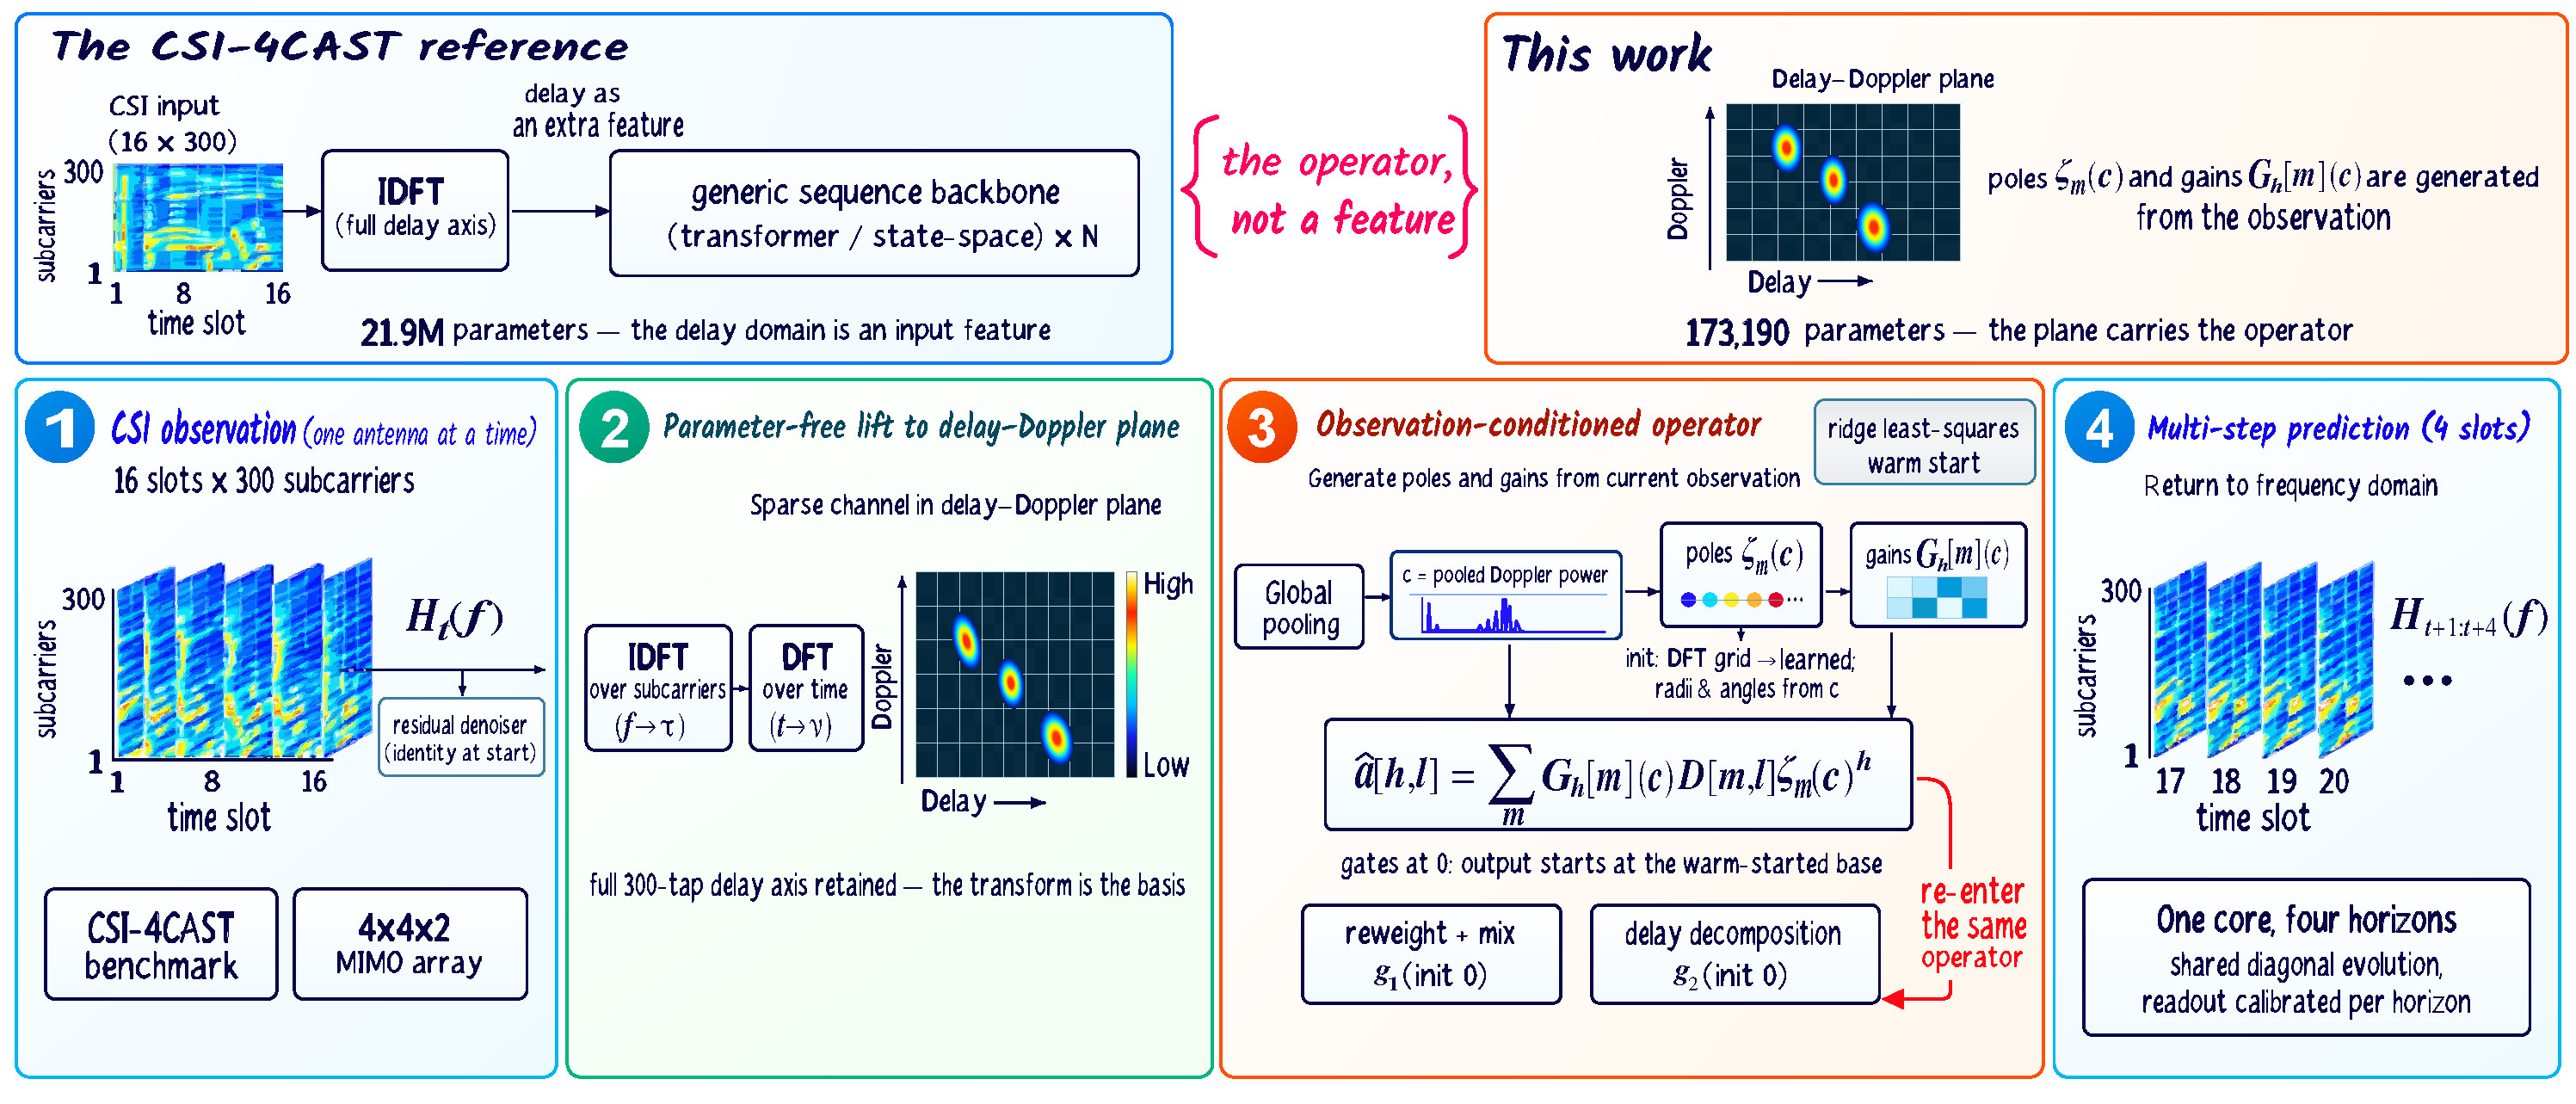
\includegraphics[width=0.91\textwidth]{fig1_final}
  \caption{Overview. The 21.9M-parameter CSI-4CAST reference attaches the
  delay domain to a generic backbone; this work puts the evolution operator
  in that plane (173,190 parameters). (1) A residual denoiser, starting as
  the identity, cleans each antenna's history. (2) A parameter-free
  IDFT/DFT lift exposes the sparse delay--Doppler spectrum. (3) A pooled
  context generates the poles $\zeta_m(\cc)$ and gains $G_h[m](\cc)$; two
  residual paths, gated from zero, re-enter the same operator. (4) The model predicts the next four slots.}
  \label{fig:arch}
\end{figure*}

\section{Experiments}
\label{sec:exp}

\subsection{Setup}
\label{ssec:setup}

The training grid has 27 subsets (3 channel models $\times$ 3 delay spreads
$\times$ 3 speeds), 24{,}300 training and 2{,}700 validation samples. The
test splits are the \emph{regular} split of 162 settings (channel model
$\times$ delay spread $\times$ speed $\times$ six signal-to-noise ratios
(SNRs)) and the \emph{robustness} split of 486 settings (phase/burst
noise and packet drops crossed with the 27 regular combinations). The
\emph{generalization} slice has 432 settings over 72 combinations drawn
from channel models B and E, with delay spreads 50/200/400\,ns and speeds
3--42\,m/s, all absent from training; the metric is the benchmark's mean
NMSE over the four horizons. For paired
statistics we
first average NMSE over the six SNR settings within each
channel-model--delay--speed cell, then bootstrap the paired cell
differences (5{,}000 resamples, 95\% CI); the intervals describe variation
across channel cells for fixed checkpoints. We train with batch 32, Adam~\cite{kingma2015adam}
at $5{\cdot}10^{-4}$ with a plateau scheduler and early stopping (600
epochs for the reported configuration, 240 for the ablation table), three
seeds.

\begin{table}[!t]
\centering
\scriptsize
\renewcommand{\arraystretch}{1.05}
\setlength{\tabcolsep}{2.8pt}
\caption{Mean NMSE on the official 162-setting grid. Published rows
(including the classical predictors) come from the benchmark's reference
table; all other rows were trained, or for the DFT-grid extrapolator
fitted without training, and scored through the same harness. $\times$ is
the ratio to the published row; Budget is the training-epoch cap. MACs
per antenna history of size $16{\times}300$: 804.9M (reference), 6.51M
(ours), 2857.0M (MambaCSP port), 15.48M (shrunk), 0.48M, 0.77M and 0.92M
(transformer rows), 73.77M (TSMixer-L), 0.58M (MLP); the DFT-grid row
counts learned MACs only, excluding its analytical FFT cost.}
\label{tab:main}
\begin{tabular}{lrrrr}
\toprule
Model & Params & Budget & NMSE & $\times$ \\
\midrule
CSI-4CAST (published)~\cite{csi4cast_2025} & 21{,}913{,}750 & --- & \textbf{0.1246} & 1.00 \\
LLM4CP (published)~\cite{llm4cp_2024} & --- & --- & 0.1413 & 1.13 \\
no prediction (published) & --- & --- & 1.8081 & 14.51 \\
DFT-grid extrap.\ (zero-train) & 0 & --- & 1.3771 & 11.05 \\
\midrule
\textbf{ours, mean of 3 seeds} & 173{,}190 & 600 ep & \textbf{0.1402} & 1.13 \\
ours, fixed-grid retrained (3 seeds) & 173{,}190 & 600 ep & 0.1401 & 1.12 \\
\midrule
MambaCSP (port, plateau) & 881{,}604 & 100 ep & 0.1468 & 1.18 \\
CSI-4CAST shrunk (91k) & 91{,}410 & 240 ep & 0.1807 & 1.45 \\
Transformer (262k) & 262{,}432 & 240 ep & 0.1891 & 1.52 \\
capacity-matched TF & 149{,}560 & 240 ep & 0.2106 & 1.69 \\
TSMixer-L~\cite{tsmixer_2023} & 124{,}337 & 240 ep & 0.2177 & 1.75 \\
PatchTST~\cite{patchtst_2023} & 616{,}560 & 240 ep & 0.2190 & 1.76 \\
MLP & 580{,}800 & 240 ep & 0.3143 & 2.52 \\
\bottomrule
\multicolumn{5}{@{}p{\columnwidth}@{}}{\rule{0pt}{1.6ex}
Re-implemented rows are single seed and early-stopped inside their budgets
under the shared validation rule; the fixed-grid retrained row retrains
the reported architecture with its offsets pinned to the DFT grid (three
seeds, \S\ref{ssec:ablations}); the MambaCSP port stopped at its
validation plateau (last improvement at epoch 93 of 100). The remaining
ports appear in the text.}
\end{tabular}
\end{table}

\subsection{Main comparison and capacity controls}
\label{ssec:main}

Table~\ref{tab:main} and Fig.~\ref{fig:pareto} give the trade-off. Our
three-seed mean NMSE is 0.1402 against the published model's 0.1246 (the
seeds score 0.1385, 0.1442 and 0.1378); the per-seed paired differences
over the 27 channel cells are $+0.0139$, $+0.0196$ and $+0.0132$, each
paired 95\% CI entirely above zero.

The benchmark's
classical predictors bound what fixed assumptions deliver: path-delay
(0.2300 in distribution) collapses to 0.3231 under shift;
autoregressive (0.7874) and Wiener (0.8236) degrade to 1.0469 and
1.0862 against the released checkpoint's 0.2872; and the fixed
16-point DFT-grid extrapolator the operator replaces reaches only
1.3771, 1.2465 and 1.2790.

We train two compact controls to test whether shrinking the published architecture or a small transformer reproduces this accuracy (Table~\ref{tab:main}, bottom). Shrinking the published architecture to
91{,}410 parameters and training it to convergence yields 0.1807, still
1.29$\times$ our three-seed mean; a transformer sized to match our
parameters reaches 0.2106. The MambaCSP port, trained for 100 epochs to
its validation plateau, remains behind the reported model on all three
splits (0.1468, 0.2796 and 0.1805) with 5.1$\times$ our parameters, so
the shift comparison does not rest on an under-trained baseline. The
remaining re-implemented ports trail further: GRU 0.3239, TCN 0.8353 and
DLinear 0.7941 among the generic families, Mamba 0.3011, iTransformer
0.3877 and TimeMixer 0.5814 among the forecasting ports. Within
our own architecture, accuracy is width-insensitive (0.1367--0.1423 across a $5.6\times$, 58k--327k parameter scan), while halving
the training windows costs about 17\% NMSE: over the tested range,
performance is more sensitive to data than to width. Both controls match our parameter scale, not our architecture.

\begin{figure}[t]
  \centering
  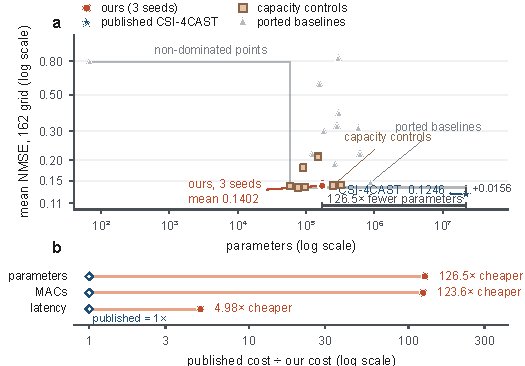
\includegraphics[width=\columnwidth]{fig_pareto}
  \caption{The accuracy--efficiency plane on the 162-setting grid (log
  scales): the reported model is the three-seed-validated operating
  point; the alternative architectures do not reach its accuracy.
  Star: published model; dots: the three reported seeds; squares: capacity
  controls (91k shrunk architecture, parameter-matched transformer, 58k--327k capacity scan); triangles: re-implemented baselines. The step
  line connects the non-dominated points; the 77k square is a single
  seed, the reported point three-seed-validated.
  Panel b: the same trade in MACs and latency.}
  \label{fig:pareto}
\end{figure}

\subsection{Behaviour under distribution shift}
\label{ssec:shift}

We evaluate three frozen checkpoints of the reported configuration on the
two shifted splits: on the 432-setting generalization slice the three
seeds score 0.2685, 0.2767 and 0.2695 against the released checkpoint's 0.2872. Each paired
difference has a 95\% CI entirely below zero ($-0.0187$, $-0.0105$,
$-0.0177$), and the three-seed mean difference is $-0.0156$
$[-0.0250,-0.0070]$ over 72 channel cells (5{,}000-resample bootstrap).
On model B the operator leads on all three seeds
(three-seed paired difference $-0.0400$, 95\% CI $[-0.0531,-0.0271]$). On
model E the released checkpoint stays ahead ($+0.0088$ $[+0.0046,+0.0132]$), though its NMSE is an order of magnitude smaller. The advantage that holds on both unseen models
is mobility: below 10\,m/s the three-seed difference is $-0.0204$
$[-0.0378,-0.0057]$; above 30\,m/s the two are indistinguishable
($+0.0001$, CI $[-0.0180,+0.0169]$).

On the same slice the shrunk architecture scores 0.3039 and the
capacity-matched transformer 0.3427, both paired CIs entirely above
zero; the plateau-trained MambaCSP port scores 0.2796 ($-0.0076$, CI
$[-0.0178,+0.0019]$) and the with-loss variant 0.2951, neither
significant.

On the benchmark's 486-setting robustness split the released checkpoint leads
consistently: 0.1623 against 0.1772, 0.1735 and 0.1777 across the three
seeds, with per-setting paired differences of $+0.0112$ to $+0.0154$.

On a second shift axis (channel models A, C and D evaluated outside
their training delay-spread and speed ranges; TDD only) the operator
stays ahead on the mean, 0.2031 against the published 0.2182
($-0.0151$, 95\% CI $[-0.0256,-0.0054]$), with the gain concentrated at
400\,ns and heterogeneous across conditions.

\subsection{Ablations and the off-grid mechanism}
\label{ssec:ablations}

\begin{table}[!t]
\centering
\scriptsize
\renewcommand{\arraystretch}{1.0}
\setlength{\tabcolsep}{7pt}
\caption{Loss-off factorial on the official grid (spectral loss off, 240
epochs, seed 42; \checkmark\ = active, off = removed). Deltas are
computed from the tabulated NMSEs.}
\label{tab:factorial}
\begin{tabular}{lccrrr}
\toprule
denoiser & decomp. & poles & NMSE & $\Delta$ & $\Delta$\,\% \\
\midrule
\checkmark & \checkmark & \checkmark & 0.1397 & --- & --- \\
\checkmark & \checkmark & off & 0.1408 & $+0.0011$ & $+0.8\%$ \\
\checkmark & off & \checkmark & 0.1425 & $+0.0028$ & $+2.0\%$ \\
\checkmark & off & off & 0.1458 & $+0.0061$ & $+4.4\%$ \\
off & \checkmark & \checkmark & 0.1779 & $+0.0382$ & $+27.3\%$ \\
off & \checkmark & off & 0.1853 & $+0.0456$ & $+32.6\%$ \\
off & off & off & 0.1862 & $+0.0465$ & $+33.3\%$ \\
off & off & \checkmark & 0.1968 & $+0.0571$ & $+40.9\%$ \\
\bottomrule
\end{tabular}
\end{table}

\textbf{Module factorial.} Table~\ref{tab:factorial} runs the full $2^3$
loss factorial. The residual denoiser is the dominant single effect
($+31.7\%$ average main effect across the four flip pairs), and removing
the denoiser together with either other module costs more than the sum
of the parts: the components complement rather than duplicate. One
implementation choice is not load-bearing (removing the least-squares
warm start costs $0.9\%$). An auxiliary squared spectral
error on the DFT of the four-horizon prediction (a squared variant of
FreDF's frequency-domain supervision~\cite{fredf_2025}) reweights the
same regression by Parseval's identity, yet every matched comparison
trains worse with it than without it (two seeds at 600 epochs, one at
240 epochs); we drop the objective.

\textbf{What the off-grid freedom is worth.} A zero-training intervention
replaces the frozen model's total learned offsets $\varepsilon_m(\cc)$ by
constants, every weight unchanged. Setting $\varepsilon_m(\cc) = 0$ snaps every pole exactly onto
the classical 16-point grid and degrades the official grid from 0.1385 to
0.1923 ($+38.8\%$) with all 162 settings worse, and every constant
global offset is worse still: the gain is per-mode, per-sample
placement.
For $|\varepsilon-\widetilde{\varepsilon}|<1$ and $h\le4$ the phase factor
of Corollary~1 is monotone in $h$, and the aggregate penalty rises
monotonically despite radius attenuation:
$+23.0/+31.1/+40.5/+45.2\%$ at h1--h4. The offsets must also be resolved finely and jointly
($1/8$-bin quantisation costs $0.9\%$, quarter-bin $5.5\%$, half-bin
$12.0\%$, keeping only the eight largest modes $17.1\%$), tracking
\eqref{eq:sensitivity}. The
same intervention degrades all 1{,}728 settings across the four splits ($+17.7\%$ to $+38.8\%$), and a 57{,}894-parameter variant loses $37.0\%$; on every shifted slice it pushes the operator below the published model ($+0.0288$ to $+0.0691$, all CIs entirely above zero). The frozen predictor's shift advantage therefore relies on its learned off-grid placement, and the placement matters at every capacity we tested (the intervention costs $37$--$60\%$ from 58k to 173k parameters).
Retraining the same architecture with the offsets pinned to the DFT
grid recovers the reported configuration (0.1401 against 0.1402
regular; 0.2688 against 0.2716 unseen, paired CI $[-0.0037,-0.0020]$,
three seeds): the calibrated transfer carries the performance; frozen
snapping measures how strongly the fitted parameterization leans on the
off-grid freedom. On the unseen slice the same
factorial attributes the shift advantage to the residual denoiser
($+20.9\%$ without it, 95\% CI $[+0.0431,+0.0713]$) and secondarily
to the delay decomposition ($+4.0\%$); removing the pole conditioning
slightly helps ($-0.9\%$).

\subsection{Efficiency}
\label{ssec:efficiency}

The reported model carries 173{,}190 parameters and 6{,}514{,}464 MACs per
antenna sample against the published
21{,}913,750 and 804{,}901,376: 126.5$\times$ and 123.6$\times$
ours. MACs are counted over matmul and convolution only; the
parameter-free DFT/IDFT lift and elementwise products are excluded. Forward latency (RTX 4090 D, batch 32, fp32; 3 warm-ups, 12
synchronised repeats, $\pm$ = s.d.\ over repeats) is
$2.24\pm0.05$\,ms against
$11.15\pm0.02$\,ms per scene, a measured scene-level speedup of
4.98$\times$; the MAC count is architectural and does not
measure wall-clock time. On the same protocol the MambaCSP port costs
9.88\,ms per scene and the capacity-matched transformer 0.40\,ms, with
NMSE 0.2106 against our 0.1402 seed mean. With
MRT beamforming the released checkpoint retains more of the perfect-CSI
rate than ours (2.06\% vs.\ 2.70\% loss, paired $+0.64$\,pp); system-level
rate remains a complementary endpoint.

\section{Conclusion}
\enlargethispage{2\baselineskip}
\label{sec:conc}

DD-Koopman replaces a generic 21.9M-parameter backbone with explicit
delay--Doppler evolution: a 173{,}190-parameter predictor with a diagonal
core, ridge-warm-started from a spectral fit
on the grid. The error analysis separates input, propagation and readout
contributions, while the ablations identify input denoising as the
dominant empirical component and reveal the strong sensitivity of the
fitted off-grid parameterization. The result: 126.5$\times$ fewer
parameters, 4.98$\times$ lower latency, and the three-seed
unseen-propagation advantage.

\clearpage

\bibliographystyle{IEEEbib}
\bibliography{references}

\end{document}
